\documentclass[11pt]{article}
    \title{\textbf{Math 217 Homework I}}
    \author{Khac Nguyen Nguyen}
    \date{}
    
    \addtolength{\topmargin}{-3cm}
    \addtolength{\textheight}{3cm}
    
\usepackage{amsmath}
\usepackage{mathtools}
\usepackage{amsthm}
\usepackage{amssymb}
\usepackage{pgfplots}
\usepackage{xfrac}
\usepackage{hyperref}
\usepackage{graphicx}
\graphicspath{ {./images/} }

\newtheorem{definition}{Definition}[section]
\newtheoremstyle{mystyle}%                % Name
  {}%                                     % Space above
  {}%                                     % Space below
  {\itshape}%                                     % Body font
  {}%                                     % Indent amount
  {\bfseries}%                            % Theorem head font
  {}%                                    % Punctuation after theorem head
  { }%                                    % Space after theorem head, ' ', or \newline
  {\thmname{#1}\thmnumber{ #2}\thmnote{ (#3)}}%                                     % Theorem head spec (can be left empty, meaning `normal')
\usepackage{tikz-qtree}

\theoremstyle{mystyle}
\newtheorem{theorem}{Theorem}[section]
\theoremstyle{definition}
\newtheorem*{exmp}{Example}
\begin{document}
\section*{1.}
First, let's establish that 
\begin{align*}
  \sum_{i=1}^n - (x_i / D) \cdot \log_2(x_i/D) 
  &= - \frac{\sum_{i=1}^n x_i \cdot (\log_2(x_i) - \log_2(D))}{N} \\
  &= -\frac{\sum_{i=1}^n x_i \cdot \log_2(x_i) + \log_2(N) \cdot \sum_{i=1}^n x_i}{N} \\ 
  &= -\frac{\sum_{i=1}^n x_i \cdot \log_2(x_i) + \log_2(N) \cdot N}{N} \\
  &= -\frac{\sum_{i=1}^n x_i \cdot \log_2(x_i)}{N} + \log_2(N) \\
\end{align*}
where $n$ is the number of categories, $N$ is the total points of data and $x_i$ is the count of each categories. 
\subsection*{1.}
\[
  H(G) = - \frac{3 \cdot \log_2(3) + 6 \cdot \log_2(6)}{9} + \log_2(9) = 0.918 
\]
\subsection*{2.}
Since there is only True label when $S$= Small. 
\[
  H(G|S=\text{Small}) = - 3 \cdot \log_2(3) / 3 + \log_2(3) = 0
\]
\subsection*{3.}
\[
  H(G|S = \text{Medium or Large}) = -\frac{3 \cdot \log_2(3) + 3 \cdot \log_2(3)}{6} + \log_2(3) = 1 
\]
\subsection*{4.}
There is 3 Small and 6 Not Small. Thus 
\[
  IG(S = \text{Small}) = H(G) - 3/9 \cdot H(G|S = \text{Small}) - 6/9 \cdot H(G|S = \text{Medium or Large}) = 
 0.251
\]
\subsection*{5.} 
There is 3 Sizes, 2 Colors, 2 Horn Types, thus there is $3 + 1 + 1= 5$ split we must consider as this is a binary decision tree. Since $S = Small$ split has only 3 True, if there is a better split (havirg higher information gain), then it must contain $\ge$ 4 True or $\ge$ 4 false. But there is no such split, thus $S$ = Small is the best split. 
\subsection*{6.}
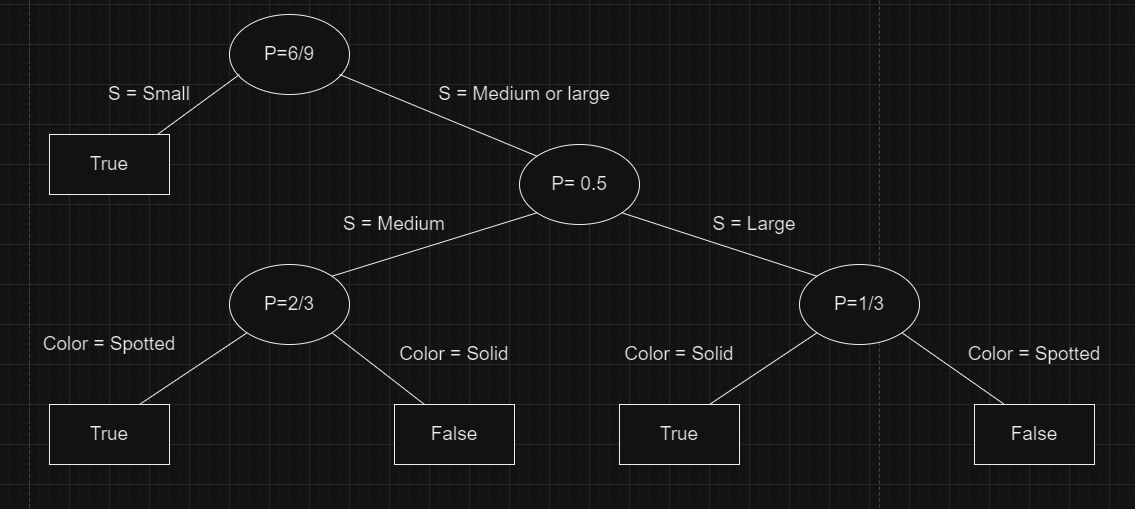
\includegraphics[scale=0.5]{BDT.png}
\section*{2.}
\subsection*{1.}
Since it is binary, that is 
\[
  p(c=1) + p(c=0) = 1
\]
We have that 
\[
  p(c=1) = \frac{\sum_{i=1}^N 1_{c_i = 1}}{N}
\]
where $N$ is the total number of data points and $\sum_{i=1}^N 1_{c_i = 1}$ is the number of data points having $c_i = 1$.  
\subsection*{2.}
$\mu_j$ is a vector in $\mathbb{R}^d$, where the $i$-th index is the mean of the $i$-th index of all the data points $x_i$ that has $c_i = j$. We have that  
\[
  \mu_j = 
  \frac{\sum_{i=1}^N 1_{c_i = j} \cdot x_i }{\sum_{i=1}^N 1_{c_i = j}}
  =
  \frac{1}{\sum_{i=1}^N 1_{c_i = j}}
  \sum_{i=1}^N
  1_{c_i = j}
  \begin{bmatrix}
    x_{i,1} \\
    x_{i,2} \\
    \vdots \\
    x_{i,d}
  \end{bmatrix} 
  = 
  \frac{1}{\sum_{i=1}^N 1_{c_i = j}}
  \begin{bmatrix}
  \sum_{i=1}^N
    1_{c_i = j} \cdot 
    x_{i,1} \\
  \sum_{i=1}^N 
    1_{c_i = j} \cdot 
    x_{i,2} \\
    \vdots \\
  \sum_{i=1}^N 
    1_{c_i = j} \cdot 
    x_{i,d}
  \end{bmatrix} 
\]
and from assumption that every variable are independent of each other. We have that 
\[
  \Sigma_j = 
  \begin{bmatrix}
    a_{j,1} & 0 & 0 & 0 \\ 
    0 & a_{j,2} & 0 & 0 \\
    0 & 0 & a_{j,3} & 0 \\
    0 & 0 & 0 & a_{j,4}
  \end{bmatrix}
\]
where 
\[
  a_{j,k} = \sum_{i=1}^N 1_{c_i = j} \cdot \frac{\sum_{i=1}^N (x_{i,k} - \mu_{j,k} )^2}{\sum_{i=1}^N 1_{c_i = j}}
\]
\subsection*{c.}
We need means and the covariance matrices to estimate the NB models because of the formula. 
\[
  G(x, \mu, \Sigma) = \displaystyle\frac{1}{\sqrt{(2\pi)^d |\Sigma|}} \exp\left( -\displaystyle\frac{1}{2} (x-\mu)^T \Sigma^{-1} (x-\mu) \right)
\]
Having means and the covariance matrices are enough to evaluate that as $x$ is the data point we want to evaluate. Without the assumption that every variables are independent of each other, the covariance matrices will not always be diagonal as the covariance of some pair of variables will be non-zero. This will makes computation much harder as well as the inverse of the covariance matrices are not guaranteed. 
\end{document}
